\PassOptionsToPackage{unicode=true}{hyperref} % options for packages loaded elsewhere
\PassOptionsToPackage{hyphens}{url}
%
\documentclass[ignorenonframetext,]{beamer}
\usepackage{pgfpages}
\setbeamertemplate{caption}[numbered]
\setbeamertemplate{caption label separator}{: }
\setbeamercolor{caption name}{fg=normal text.fg}
\beamertemplatenavigationsymbolsempty
\usepackage{lmodern}
\usepackage{amssymb,amsmath}
\usepackage{ifxetex,ifluatex}
\usepackage{fixltx2e} % provides \textsubscript
\ifnum 0\ifxetex 1\fi\ifluatex 1\fi=0 % if pdftex
  \usepackage[T1]{fontenc}
  \usepackage[utf8]{inputenc}
  \usepackage{textcomp} % provides euro and other symbols
\else % if luatex or xelatex
  \usepackage{unicode-math}
  \defaultfontfeatures{Ligatures=TeX,Scale=MatchLowercase}
\fi
\usetheme[]{CambridgeUS}
\usecolortheme{beaver}
\usefonttheme{structurebold}
% use upquote if available, for straight quotes in verbatim environments
\IfFileExists{upquote.sty}{\usepackage{upquote}}{}
% use microtype if available
\IfFileExists{microtype.sty}{%
\usepackage[]{microtype}
\UseMicrotypeSet[protrusion]{basicmath} % disable protrusion for tt fonts
}{}
\IfFileExists{parskip.sty}{%
\usepackage{parskip}
}{% else
\setlength{\parindent}{0pt}
\setlength{\parskip}{6pt plus 2pt minus 1pt}
}
\usepackage{hyperref}
\hypersetup{
            pdftitle={B1 - Das Arbeiten mit OSM Daten},
            pdfauthor={Jan-Philipp Kolb},
            pdfborder={0 0 0},
            breaklinks=true}
\urlstyle{same}  % don't use monospace font for urls
\newif\ifbibliography
\usepackage{graphicx,grffile}
\makeatletter
\def\maxwidth{\ifdim\Gin@nat@width>\linewidth\linewidth\else\Gin@nat@width\fi}
\def\maxheight{\ifdim\Gin@nat@height>\textheight\textheight\else\Gin@nat@height\fi}
\makeatother
% Scale images if necessary, so that they will not overflow the page
% margins by default, and it is still possible to overwrite the defaults
% using explicit options in \includegraphics[width, height, ...]{}
\setkeys{Gin}{width=\maxwidth,height=\maxheight,keepaspectratio}
% Prevent slide breaks in the middle of a paragraph:
\widowpenalties 1 10000
\raggedbottom
\setbeamertemplate{part page}{
\centering
\begin{beamercolorbox}[sep=16pt,center]{part title}
  \usebeamerfont{part title}\insertpart\par
\end{beamercolorbox}
}
\setbeamertemplate{section page}{
\centering
\begin{beamercolorbox}[sep=12pt,center]{part title}
  \usebeamerfont{section title}\insertsection\par
\end{beamercolorbox}
}
\setbeamertemplate{subsection page}{
\centering
\begin{beamercolorbox}[sep=8pt,center]{part title}
  \usebeamerfont{subsection title}\insertsubsection\par
\end{beamercolorbox}
}
\AtBeginPart{
  \frame{\partpage}
}
\AtBeginSection{
  \ifbibliography
  \else
    \frame{\sectionpage}
  \fi
}
\AtBeginSubsection{
  \frame{\subsectionpage}
}
\setlength{\emergencystretch}{3em}  % prevent overfull lines
\providecommand{\tightlist}{%
  \setlength{\itemsep}{0pt}\setlength{\parskip}{0pt}}
\setcounter{secnumdepth}{0}

% set default figure placement to htbp
\makeatletter
\def\fps@figure{htbp}
\makeatother


\title{B1 - Das Arbeiten mit OSM Daten}
\author{Jan-Philipp Kolb}
\date{22 Oktober 2018}

\begin{document}
\frame{\titlepage}

\begin{frame}{Inhalt dieses Abschnitts}
\protect\hypertarget{inhalt-dieses-abschnitts}{}

\begin{itemize}
\tightlist
\item
  Vorstellung des Openstreetmap (OSM) Projekts
\item
  Welche OSM-Daten sind erhältlich?
\item
  Vorstellung von Forschung die mit OSM-Daten durchgeführt wurde
\end{itemize}

\end{frame}

\begin{frame}{\href{http://www.openstreetmap.de/}{OpenStreetMap}
Projekt}
\protect\hypertarget{openstreetmap-projekt}{}

\begin{quote}
OpenStreetMap.org ist ein im Jahre 2004 gegründetes internationales
Projekt mit dem Ziel, eine freie Weltkarte zu erschaffen. Dafür sammeln
wir weltweit Daten über Straßen, Eisenbahnen, Flüsse, Wälder, Häuser und
vieles mehr.
\end{quote}

\url{http://www.openstreetmap.de/}

\end{frame}

\begin{frame}{OpenStreetMap}
\protect\hypertarget{openstreetmap}{}

\begin{quote}
OpenStreetMap (OSM) ist ein kollaboratives Projekt um eine editierbare
Weltkarte zu erzeugen.
\end{quote}

\href{https://en.wikipedia.org/wiki/OpenStreetMap}{\textbf{Wikipedia -
OpenStreetMap}}

\end{frame}

\begin{frame}{\href{http://wiki.openstreetmap.org/wiki/DE:Map_Features}{OSM
Map Features}}
\protect\hypertarget{osm-map-features}{}

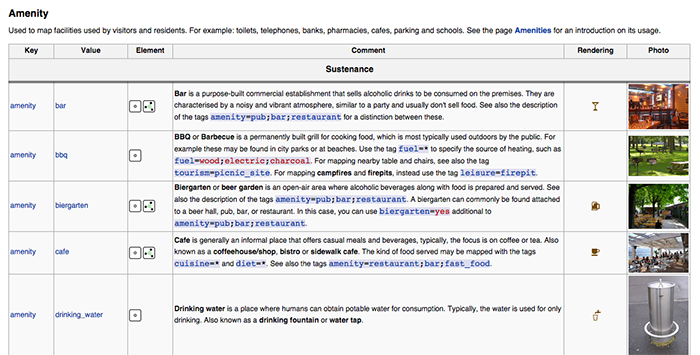
\includegraphics{figure/osm_mapfeatures.png}

\end{frame}

\begin{frame}{\href{https://wiki.openstreetmap.org/wiki/Tags}{Openstreetmap
Tags}}
\protect\hypertarget{openstreetmap-tags}{}

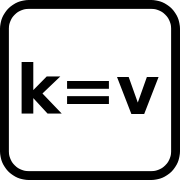
\includegraphics{figure/osm_tag.png}

\end{frame}

\begin{frame}{Objekttypen in OSM}
\protect\hypertarget{objekttypen-in-osm}{}

\begin{itemize}
\item
  Es gibt prinipiell drei verschiedene Objekttypen:
\item
\end{itemize}

\end{frame}

\begin{frame}{Download von OpenStreetMap Daten}
\protect\hypertarget{download-von-openstreetmap-daten}{}

\begin{itemize}
\item
  \url{https://mapzen.com/} - Ausschnitte von OpenStreetMap für einzelne
  Städte (\href{https://mapzen.com/data/metro-extracts/}{metro
  extracts})
\item
  Über Geofabrik lassen sich aktuelle Ausschnitte (auch Shapefiles)
  herunterladen (\url{http://download.geofabrik.de/})
\item
  Kartendaten (\href{http://www.openaprs.net/}{\textbf{openaprs}})
\end{itemize}

\end{frame}

\begin{frame}[fragile]{Bei großen Datenmengen}
\protect\hypertarget{bei-groen-datenmengen}{}

\begin{itemize}
\item
  Hier geht es nur um das Herunterladen kleiner Ausschnitte.
\item
  Wenn größere Datenmengen benötigt werden, sollte man eine
  Datenbanklösung finden.
\item
  \href{http://www.postgresql.org/}{PostgreSQL} hat den Vorteil, dass es
  Open-Source ist.
\item
  \href{http://www.postgresql.org/download/windows/}{Download PostreSQL}
\item
  \href{https://datashenanigan.wordpress.com/2015/05/18/getting-started-with-postgresql-in-r/}{Hier}
  ist eine Einführung in PostgreSQL zu finden
\item
  Sehr empfehlenswert: Arbeiten mit pgAdmin III
\item
  Beispiel: um Verknüpfung zu einer Datenbank herzustellen - Doppelklick
  auf den Server in pgAdmin III
\end{itemize}

\begin{block}{PostGIS für PostgreSQL}

\begin{itemize}
\tightlist
\item
  \href{http://postgis.net/install/}{\textbf{Installieren}} der PostGIS
  Erweiterung:
\end{itemize}

\begin{verbatim}
CREATE EXTENSION postgis;
\end{verbatim}

\end{block}

\end{frame}

\begin{frame}[fragile]{Programm zum Import der OSM Daten in PostgreSQL-
osm2pgsql}
\protect\hypertarget{programm-zum-import-der-osm-daten-in-postgresql--osm2pgsql}{}

\begin{itemize}
\tightlist
\item
  Läuft unter Linux deutlich besser
\item
  so könnte bspw. ein Import in PostgreSQL aussehen:
\end{itemize}

\begin{verbatim}
osm2pgsql -c -d osmBerlin --slim -C  -k  berlin-latest.osm.pbf
\end{verbatim}

\end{frame}

\begin{frame}{Nutze bspw. \href{http://www.qgis.org/de/site/}{QGIS} um
Shapefiles zu extrahieren}
\protect\hypertarget{nutze-bspw.-qgis-um-shapefiles-zu-extrahieren}{}

\begin{itemize}
\tightlist
\item
  \href{http://www.qgistutorials.com/de/docs/downloading_osm_data.html}{Plugin
  OpenLayers}
\end{itemize}

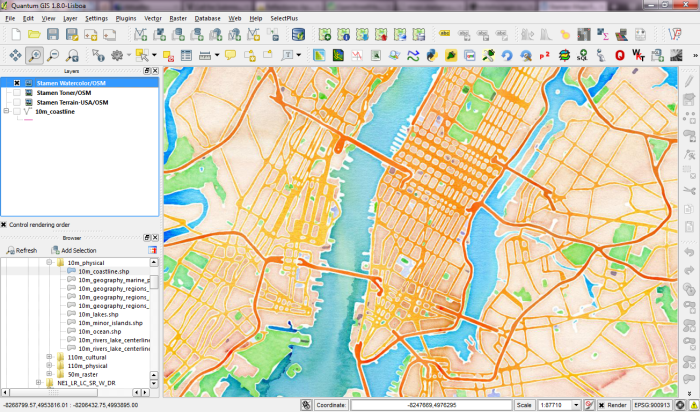
\includegraphics{figure/stamen_watercolor1.png}

\end{frame}

\begin{frame}{Links}
\protect\hypertarget{links}{}

\begin{itemize}
\item
  \href{http://wiki.openstreetmap.org/wiki/Downloading_data}{\textbf{Wiki
  zum Downlaod}} von Openstreetmap Daten
\item
  \href{http://blog.openstreetmap.de/}{\textbf{Openstreetmap Blog}}
\item
  Liste möglicher Datenquellen für räumliche Analysen
  (\href{http://wiki.openstreetmap.org/wiki/Potential_Datasources}{weltweit}
  und in
  \href{http://wiki.openstreetmap.org/wiki/DE:Potential_Datasources}{\textbf{Deutschland}}
  )
\item
  \href{http://wiki.openstreetmap.org/wiki/SALB}{\textbf{SALB}} -
  Administrative Grenzen
\end{itemize}

\url{http://wiki.openstreetmap.org/wiki/SALB}

\end{frame}

\end{document}
